\documentclass[11pt,letterpaper]{article}
\usepackage[utf8]{inputenc}
\usepackage[letterpaper,includeheadfoot, top=0.5cm, bottom=3.0cm, right=1.5cm, left=1.5cm]{geometry}
\renewcommand{\familydefault}{\sfdefault}
\usepackage{float} % Allows putting an [H] in \begin{figure} to specify the exact location of the figure
\renewcommand{\figurename}{Fig.}
\usepackage{lmodern}% http://ctan.org/pkg/lm
\usepackage{amsmath}
\usepackage{graphicx}
\usepackage{color}
\usepackage{amssymb}
\usepackage{url}
\usepackage{pdfpages}
\usepackage{fancyhdr}
\usepackage{subfig}
\usepackage{listings} %Codigo
\usepackage{selinput}                   % Compatibilidad con acentos
\usepackage[colorlinks = true,
            linkcolor = blue,
            urlcolor  = blue,
            citecolor = blue,
            anchorcolor = blue]{hyperref}
\newcommand{\bR}{\ensuremath{\mathbb{R}}}
\newcommand{\bN}{\ensuremath{\mathbb{N}}}
\newcommand{\bZ}{\ensuremath{\mathbb{Z}}}
\newcommand{\bP}{\ensuremath{\mathbb{P}}}
\newcommand{\bE}{\ensuremath{\mathbb{E}}}
\newcommand{\bD}{\ensuremath{\mathbb{D}}}
\newcommand{\bV}{\ensuremath{\mathbb{V}}}
\newcommand{\cN}{\ensuremath{\mathcal{N}}}
\newcommand{\x}{\ensuremath{\mathbf{x}}}
\newcommand{\m}{\ensuremath{\mathbf{m}}}
\newboolean{pauta}
\setboolean{pauta}{false}
%\usepackage{tkz-graph}
%\usetikzlibrary{arrows}
%\usepackage{algorithm}
%\usepackage{algorithmic}

\lstset{language=C, tabsize=4,framexleftmargin=5mm,breaklines=true}

\begin{document}

% ·············· ENCABEZADO - PIE DE PAGINA ············
\pagestyle{fancy}
\fancyhf{}
\lhead{\textbf{MA5204: Aprendizaje de Máquinas 2020}}
\rfoot{Page \thepage}
%Encabezado

% =============== Inicio Documento ===============
%\rm
\headheight = 14pt
\begin{center}
\large{\textbf{Tarea 1}}
\end{center}
\textbf{Profesor:} Felipe Tobar\\
\textbf{Auxiliares:} José Díaz, Diego Garrido, Jou-Hui Ho, Luis Muñoz, Diego Troncoso \\
\textbf{Consultas:} Diego Garrido,  Diego R. Troncoso  (U-cursos)\\
\textbf{Período:} 13/4/2020 --- 20/4/2020 \\

\noindent\textbf{Formato entrega:} Informe en formato PDF, con una extensión máxima de 3 páginas (puede usar un formato de doble columna), presentando y analizando sus resultados, y detallando la metodología utilizada. Adicionalmente debe entregar el jupyter notebook (o el código que haya generado) con la resolución de la tarea.

\vspace{5mm}

\noindent\textbf{P1. Descomposición Sesgo-Varianza} \textbf{(2.0 puntos)}
\vspace{5 mm}
\begin{itemize}
    \item[(a)] (0.5 puntos) Considere el conjunto de  observaciones  $D=\{(x_{i}, y_{i})\}_{i=1}^{N}$, relacionadas mediante el modelo lineal  
    	\begin{equation*}
    	    y_{i}=\theta^\top x_{i}+\epsilon_{i},
    	\end{equation*}
    	 donde $\{\epsilon_{i}\}_{i=1}^N$ son observaciones i.i.d con $\mathbb{E}[\epsilon]=0$ y $\text{var}(\epsilon)=\sigma^{2}$,  $\theta$ es un parámetro fijo y desconocido. Para un nuevo par, denotado $(x,y)$, no contenido en el conjunto de observaciones $D$, considere la predicción de $y$ mediante $\hat y=\hat\theta^\top x$, donde $\hat{\theta}$ es un estimador del  parámetro $\theta$ basado en $D$. Muestre que el costo cuadrático esperado de predecir $y$  con $\hat y$ (recuerde que las esperanzas se toman con   respecto a la ley de $\epsilon$) admite la siguiente  descomposición sesgo-varianza:
    	\begin{equation*}
    	    \mathbb{E}\left[(\hat{y}-y)^{2}\right] = \text{var}(\hat{y})+\text{sesgo}^{2}(\hat{y}) + \sigma^{2},
    	\end{equation*}
        donde: i) el primer término es la varianza de la variable aleatoria $\hat y$, con $\text{var}(\hat{y})=\mathbb{E}\left[(\hat{y}-\mathbb{E}[\hat{y}])^{2}\right]$ (recuerde que $\hat\theta$ es variable aleatoria, pues depende de $D$), ii) el segundo término es el sesgo al cuadrado de la variable aleatoria $\hat{y}$, con $\text{sesgo}(\hat{y})=E\left[\hat{y}-y\right]=E\left[\hat{y}\right]- \theta^\top x$, y  iii) $\sigma^2$ es la varianza de $\epsilon$.

    \textbf{Solución}:\\
      
    \begin{align*}
        E\big[(\hat{y}-y)^{2}\big]&=E\big[\big((\hat{y}-E[\hat{y}])-(E[y]+\epsilon-E[\hat{y}])\big)^{2}\big] \\
        & = E\big[(\hat{y}-E[\hat{y}])^{2}\big]+E\big[(E[y]+\epsilon-E[\hat{y}])^{2}\big]-2E\big[(\hat{y}-E[\hat{y}])(E[y]+\epsilon-E[\hat{y}])\big]\\
        & = var(\hat{y})+E\big[E[y]^{2}+\epsilon^{2}+E[\hat{y}]^{2}+2\epsilon E[y]-2E[y]E[\hat{y}]-2\epsilon E[\hat{y}]\big]\\
        & - 2E\big[\hat{y}E[y]+\hat{y}\epsilon-\hat{y}E[\hat{y}]-E[\hat{y}]E[y]-E[\hat{y}]\epsilon+E[\hat{y}]^{2}\big]\\
        & = var(\hat{y})+E[y]^{2}+\sigma^{2}+E[\hat{y}]^{2}-2E[y]E[\hat{y}]-2E[\hat{y}]E[y]+2E[\hat{y}]^{2}+2E[\hat{y}]E[y]-2E[\hat{y}]^{2}\\
        & = var(\hat{y})+\sigma^{2}+E[y]^{2}+E[\hat{y}^{2}]-2E[y]E[\hat{y}]\\
        & = var(\hat{y})+sesgo^{2}(\hat{y})+\sigma^{2}
    \end{align*}

	\item[(b)] (1.0 puntos) Para los parámetros de mínimos cuadrados $\theta_{MC} = (X^\top X) ^{-1}X^\top Y $  y de  mínimos cuadrados regularizados $\theta_{MCR} = (X^\top X + \rho I) ^{-1}X^\top Y$ calcule el sesgo y la varianza de la predicción.
	
	\textbf{Solución}:\\
	\textbf{MC}
	\begin{itemize}
	    \item[(i)] \textbf{Sesgo}\\
	    \begin{align*}
	        E[\hat{y}-y] & = E[x^{T}\hat{\theta}_{MC}]-E[x^{T}\theta+\epsilon]=E[x^{T}(X^{T}X)^{-1}X^{T}Y]-x^{T}\theta \\
	        & = E\big[x^{T}(X^{T}X)^{-1}X^{T}(X\theta+\epsilon)\big]-x^{T}\theta = E[x^{T}\theta+x^{T}(X^{t}X)^{-1}X^{T}\epsilon] -x^{T}\theta\\
	        & = x^{T}\theta-x^{T}\theta = 0
	    \end{align*}
	    \item[(ii)] \textbf{Varianza}\\
	    \begin{align*}
	    E[(\hat{y}-E[\hat{y}])^{2}] & = E[\hat{y}^{2}]-E[\hat{y}]^{2} = E[(x^{T}\theta+x^{T}(X^{T}X)^{-1}X^{T}\epsilon)^{2}]-(x^{T}\theta)^{2}\\
	    & = E[(x^{T}\theta)^{2}+2x^{T}\theta w^{T}\epsilon+w^{T}\epsilon\epsilon^{T}w]-(x^{T}\theta)^{2}, w^{T} =x^{T}(X^{T}X)^{-1}X^{T}, w^{T}\epsilon=\epsilon^{T} w\\
	    & = (x^{T}\theta)^{2}+w^{T}\sigma^{2}Iw-(x^{T}\theta)^{2} = \sigma^{2}x^{T}(X^{T}X)^{-1}X^{T}X(X^{T}X)^{-1}x=\sigma^{2}x^{T}(X^{T}X)^{-1}x
	    \end{align*}
	\end{itemize}
	\textbf{MCR}
	\begin{itemize}
	    \item[(i)] \textbf{Sesgo}\\
	    \begin{align*}
	    E[\hat{y}-y] &= E[x^{T}\hat{\theta}_{MCR}]-x^{T}\theta=E[x^{T}(X^{T}X+\rho I)^{-1}X^{T}(X\theta+\epsilon)]-x^{T}\theta\\
	    & = x^{T}(X^{T}X+\rho I)^{-1}X^{T}X\theta-x^{T}\theta=x^{T}(I+\rho (X^{T}X)^{-1})^{-1}\theta-x^{T}\theta\\
	    & =  x^{T}\big[\big(I+\rho (X^{T}X)^{-1}\big)^{-1}-I\big]\theta
	    \end{align*}
	    
	    \item[(ii)]\textbf{Varianza} \\ 
	     \begin{align*}
	    E\big[(\hat{y}-E[\hat{y}])^{2}\big] & =  E[\hat{y}^{2}]-E[\hat{y}]^{2} = E\big[\big(w^{T}(X\theta+\epsilon)\big)^{2}\big]-E\big[w^{T}(X\theta+\epsilon)\big]^{2}, w^{T}=x^{T}(X^{T}X+\rho I)^{-1}X^{T}\\ 
	    & = E\big[(w^{T}X\theta)^{2}+2w^{T}X\theta\epsilon+w^{T}\epsilon\epsilon^{T}w\big]-(w^{T}X\theta)^{2}=w^{T}\sigma^{2}Iw\\
	    & = \sigma^{2}x^{T}(X^{T}X+\rho I)^{-1}X^{T}X(X^{T}X+\rho I)^{-1}x
	    \end{align*}
	\end{itemize}
	
	\item[(c)] (0.5 puntos) Analice las expresiones anteriores. ¿Cuáles son las ventajas y desventajas de ambos estimadores? ¿Qué aseveraciones  puede hacer de la comparación de ambos criterios (MC y MCR) con respecto de  sus  sesgos y  varianzas?
	
	\textbf{Solución}:\\
	
	La desventaja de MCR es que la predicción es sesgada, puesto que para $x$ y $\theta$ cualquiera la única forma de que el sesgo sea $0$ es tomando $\rho=0$, lo que resultaría en el estimador de MC. Como ventaja de MCR se tiene que la varianza de la predicción es menor que la de MC, lo que lo vuelve más robusto, siendo menos sensible a correlaciones espúreas u outliers presentes en el conjunto de entrenamiento teniendo la capacidad de generalizar mejor en conjunto de datos fuera de muestra. 
	
	Mostrar que la varianza de la predicción de MCR es menor que MC no es trivial, por tanto, debe demostrarse. Por demostrar que $var(\hat{y}_{MC})-var(\hat{y}_{MCR}) > 0$:\\

	\begin{align*}
    var(\hat{y}_{MC})-var(\hat{y}_{MCR}) & =  \sigma^{2}x^{T}(X^{T}X)^{-1}x-\sigma^{2}x^{T}W(X^{T}X)^{-1}W^{T}x,\; W=(X^{T}X+\rho I)^{-1}X^{T}X\\
    & = \sigma^{2}x^{T}W\big[W^{-1}(X^{T}X)^{-1}W^{T^{-1}}-(X^{T}X)^{-1} \big]W^{T}x\\
    & = \sigma^{2}x^{T}W\big[(X^{T}X)^{-1}(X^{T}X+\rho I)(X^{T}X)^{-1}(X^{T}X+\rho I)(X^{T}X)^{-1} -(X^{T}X)^{-1} \big]W^{T}x \\
    & = \sigma^{2}x^{T}W\big[2\rho(X^{T}X)^{-2}+\rho^{2}(X^{T}X)^{-3}\big]W^{T}x\\
    & = \sigma^{2}x^{T}[(X^{T}X+\rho I)^{-1}][2\rho I+\rho^{2}(X^{T}X)^{-1}][(X^{T}X+\rho I)^{-1}]^{T}x\\
    & = \theta^{2}x^{T}\Sigma(\rho) x >0, \;\Sigma(\rho)=[(X^{T}X+\rho I)^{-1}][2\rho I+\rho^{2}(X^{T}X)^{-1}][(X^{T}X+\rho I)^{-1}]^{T}, \; \forall \rho >0
	\end{align*}
	
	Para llegar la desigualdad de la útlima linea un pequeño repaso de algebra lineal:
	
	Una matriz semidefinida positiva $W \succeq 0$ cumple que $x^{T}Wx\geq0 \; \forall x$, si $x^{T}Wx>0 \; \forall x \neq 0$ se dice que $W$ es definida positiva $W \succ 0$. Algunas propiedades:
	
	\begin{enumerate}
	     \item $A\succeq 0, B\succeq 0 \implies  A+B\succeq 0$
	     \item $A\succ 0, B\succeq 0 \implies  A+B\succ 0$
	     \item $A\succeq 0, \lambda\geq0 \implies  \lambda A \succeq 0$
	     \item $A\succ 0, \lambda>0\implies  \lambda A \succ 0$
	     \item $A\succeq 0 \implies A^{-1}\succeq 0 $
	     \item $A\succ 0 \implies A^{-1}\succ 0 $
	     \item Si $M\succeq0$ y $Q$ tiene rango completo en las columnas $\implies Q^{T}MQ\succeq0$
 	     \item Si $M\succ0$ y $Q$ tiene rango completo en las columnas $\implies Q^{T}MQ\succ0$
 	     \item $A\succeq 0, B\succeq 0$ y $AB=BA$, entonces $AB\succeq0$
 	     \item $A\succ 0, B\succ 0$ y $AB=BA$, entonces $AB\succ0$
	\end{enumerate}
	
	La matriz $X^{T}X$ es semidefinida positiva, la matriz $I$ es definida positiva, $(X^{T}X+\rho I)^{-1}$ es definida positiva $\forall \rho>0$ (propiedad 2, 4 y 6), además  tiene rango completo en las columnas puesto que es invertible, similarmente $2\rho I+\rho^{2}(X^{T}X)^{-1}$ es definida positiva $\forall \rho>0$, luego por propiedad (8) $\Sigma(\rho)=[(X^{T}X+\rho I)^{-1}][2\rho I+\rho^{2}(X^{T}X)^{-1}][(X^{T}X+\rho I)^{-1}]^{T}$ es definida positiva $\forall \rho>0$. 
	
Otra forma de demostrar lo mismo es darse cuenta que $var(\hat{y})$ es decreciente en $\rho$, para esto debemos demostrar que su derivada es no positiva:\\
%https://math.stackexchange.com/questions/1471825/derivative-of-the-inverse-of-a-matrix

\begin{align*}
var(\hat{y})' & = -\sigma^{2}x^{T}(X^{T}X+\rho I)^{-2}X^{T}X(X^{T}X+\rho I)^{-1}x-\sigma^{2}x^{T}(X^{T}X+\rho I)^{-1}X^{T}X(X^{T}X+\rho I)^{-2}x\\
& = -\sigma^{2}x^{T}\big[(X^{T}X+\rho I)^{-1}\big((X^{T}X+\rho I)^{-1}X^{T}X+X^{T}X(X^{T}X+\rho I)^{-1}\big)(X^{T}X+\rho I)^{-1}\big]x^{T},\\
& = -\sigma^{2}x^{T}(X^{T}X+\rho I)^{-1}[2(I+\rho(X^{T}X)^{-1})^{-1}](X^{T}X+\rho I)^{-1}x^{T}\\
& =  -\sigma^{2}x^{T}\Sigma(\rho)x^{T} < 0, \; \Sigma(\rho)= (X^{T}X+\rho I)^{-1}[2(I+\rho(X^{T}X)^{-1})^{-1}](X^{T}X+\rho I)^{-1} \succ 0 \; \forall \rho >0
\end{align*}

Tenemos que $2(I+\rho(X^{T}X)^{-1})$ es definida positiva por propiedad 2 y 6, ya que $I\succ0$ y $\rho(X^{T}X)^{-1}\succeq0$. \\

\newpage
\vspace{5 mm}
\noindent\textbf{P2. Regresión Lineal} \textbf{(4.0 puntos)}
\vspace{5 mm}
\href{https://nbviewer.jupyter.org/github/dgarridoa/T1ML/blob/master/solucion.ipynb}{Solución}\\

Como primer paso debe instalar \href{https://www.anaconda.com/distribution/}{Anaconda} una distribución de Python que proporciona el stack básico de Python para la ciencia de datos, debe descargar la versión Python 3.7. Anaconda incluye  \href{https://jupyter.org/}{Jupyter Notebook}, un entorno de desarrollo interactivo web.\\

Para esta pregunta se pide implementar el estimador de mínimos cuadrados y de mínimos cuadrados regularizados con regularizador \textit{ridge} para un conjunto de datos. Para la implementación de los estimadores \textbf{solo está permitido el uso de operaciones de álgebra lineal}, para esto pueden utilizar el stack de numpy.\\

Como base de datos del experimento se utilizará el archivo \textbf{Housing.csv}, este corresponde a un dataset que posee precios de casas de algunas localidades de USA. Este dataset consta de  una variable $X$, que corresponde al ingreso promedio de la población en esa área (\textit{Avg Area Income}), e $Y$, que corresponde al precio de las casas. El objetivo de esta pregunta es aprender una función lineal que relacione $X$ e $Y$, así un agente inmobiliario que no tiene información sobre el precio de las casas en una nueva localidad pueda fijarle un precio a estas en base al ingreso promedio del área. Para una correcta comparación de los estimadores la base de datos viene dividida en dos conjuntos, entrenamiento (\textit{in-sample}) y validación (\textit{out-of-sample}).

Para esto deberá:

\begin{itemize}
	\item[(a)] (0.5 puntos) Cargar los datos desde el archivo \textbf{Housing.csv} y graficarlos.\\
	
	\begin{minipage}{\linewidth}
	    \centering
        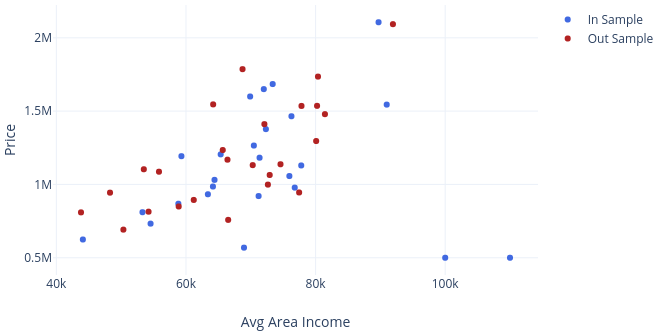
\includegraphics[width=\textwidth]{img/data.png}
	\end{minipage}
	
	\item[(b)] (1.0 puntos) Implemente el estimador de mínimos cuadrados regularizados usando regularización \textit{ridge} y obtenga el vector de parámetros $\theta$ para diferentes valores de $\rho \in [0, 10]$ incluyendo los límites. Para esto implemente la función \textit{reg\_lineal(X,Y,$\rho$)}. 
 Ejemplo de parámetros estimados para $\rho \in [0,1]$, donde $\theta_{0}$ es el intercepto y $\theta_{1}$ la pendiente.


\begin{center}
\begin{tabular}{|r|r|r|}
\hline
\textbf{$\rho$} & \textbf{$\theta_{0}$} & \textbf{$\theta_{1}$} \\ \hline
0.0             & 856479.11             & 3.62                                       \\ \hline
0.5             & 558528.88             & 7.62                                       \\ \hline
1.0             & 414376.44             & 9.55                                       \\ \hline
1.5             & 329368.67             & 10.69                                      \\ \hline
2.0             & 273301.82             & 11.44                                      \\ \hline
2.5             & 233546.35             & 11.98                                      \\ \hline
3.0             & 203888.06             & 12.37                                      \\ \hline
3.5             & 180913.64             & 12.68                                      \\ \hline
4.0             & 162592.48             & 12.93                                      \\ \hline
4.5             & 147640.86             & 13.13                                      \\ \hline
5.0             & 135207.49             & 13.29                                      \\ \hline
5.5             & 124705.59             & 13.44                                      \\ \hline
6.0             & 115717.52             & 13.56                                      \\ \hline
6.5             & 107937.97             & 13.66                                      \\ \hline
7.0             & 101138.54             & 13.75                                      \\ \hline
7.5             & 95145.00              & 13.83                                      \\ \hline
8.0             & 89822.07              & 13.90                                      \\ \hline
8.5             & 85063.18              & 13.97                                      \\ \hline
9.0             & 80783.18              & 14.02                                      \\ \hline
9.5             & 76913.25              & 14.08                                      \\ \hline
10.0            & 73397.14              & 14.12                                      \\ \hline
\end{tabular}
\end{center}

	\item[(c)] (0.5 puntos) Grafique el valor de los parámetros estimados para los valores de $\rho$.\\
	
    \begin{minipage}{\linewidth}
        \centering
        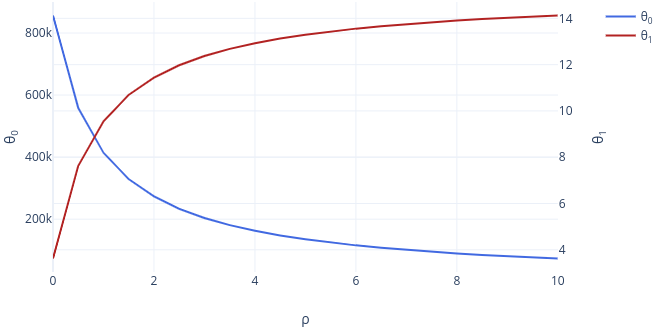
\includegraphics[width=1\textwidth]{img/params.png}
    \end{minipage}	
	\item[(d)] (0.5 puntos) Grafique el error cuadrático medio y la varianza de la predicción para los valores de $\rho$ tanto en el conjunto de entrenamiento como en el de validación.\\
	
	La varianza de la predicción no es $var(\hat{y}) = \frac{1}{N}\sum_{i=1}^{N}(\hat{y_{i}}-\bar{\hat{y}})^{2}$, si se calcula así se tendrá un curva creciente en $\rho$, se debe calcular a partir del promedio de las varianza de la predicción sobre observaciones individuales usando la formula derivada en la pregunta 1. Notar que el $\sigma^{2}$ de la formula se estima sobre los datos de entrenamiento,  por ende $\sigma^{2}$ se estima una vez para cada $\rho$.
	\end{itemize}

	\begin{minipage}{\linewidth}
    \centering
    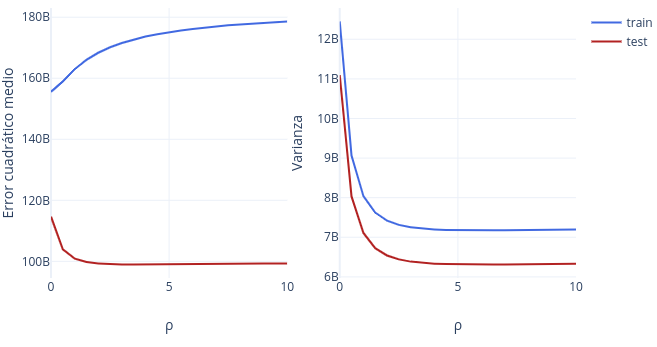
\includegraphics[width=\textwidth]{img/mse_var.png}
    \end{minipage}	
	
	\item[(e)] (0.5 puntos) Grafique la ecuación de la recta con los parámetros estimados para diferentes valores de $\rho$ junto a los datos de entrenamiento y validación.\\
	
	\begin{minipage}{\linewidth}
    \centering
    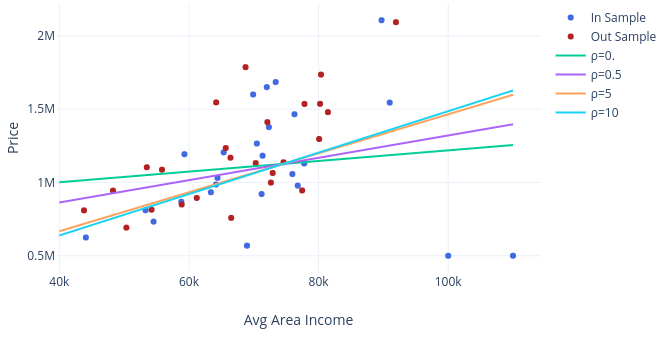
\includegraphics[width=\textwidth]{img/lines.png}
    \end{minipage}	
	
	\item[(f)] (1.0) Discuta cómo elegir  el valor apropiado de $\rho$ en base a los resultados obtenidos en los puntos anteriores.
	
Notar que de la figura del punto (b) se observa que la norma del vector de parámetros es decreciente en $\rho$, el efecto de esto se observa en (e), donde las rectas obtenidas fijando $\rho$ mayor son menos afectadas o cargadas en la dirección de los dos outliers de la esquina inferior derecha presentes en el conjunto de entrenamiento. \\

Es importante destacar que el desempeño en el conjunto de entrenamiento empeora a medida que $\rho$ aumenta y de hecho es mínimo para $\rho=0$, pero le objetivo de una tarea predictiva es obtener un modelo con alta capacidad de generalización, es decir, que tenga un buen desempeño en un conjunto de datos no visto en entrenamiento, en este caso $\rho$ puede calibrarse de tal manera que la disminución de la varianza de la predicción compense el incremento del sesgo al cuadrado, pudiendo tener un error cuadrático medio (nuestra médida de desempeño escogida) igual o menor al obtenido por MC en un conjunto de validación, para los $\rho$ probados el error cuadrático medio alcanza su valor mínimo en $\rho=3.5$. \\

Notar que buscar $\rho$ que minimice la varianza de la predicción no está bien, ya que si tomamos $\rho=\infty \implies \theta=0 \implies var(\hat{y})=0$, luego se tiene que la varianza es mínima y el error cuadrático medio es máximo.

\end{itemize}

 \textbf{No} se permite el uso de paquetes predefinidos para regresión lineal. Estos pueden ser considerados para contrastar los propios resultados pero no para resolver la pregunta. E.g., \texttt{numpy.polyfit},  \texttt{scipy.stats.linregress}, \texttt{sklearn.linear\_model.LinearRegression}.

\end{document}


